\documentclass[11pt]{article}
\usepackage{amssymb}
\usepackage{algorithm}  
\usepackage{algpseudocode}  
\usepackage{amsmath}  
\usepackage{graphicx}
\renewcommand{\algorithmicrequire}{\textbf{Input:}}  % Use Input in the format of Algorithm  
\renewcommand{\algorithmicensure}{\textbf{Output:}}
\parindent=22pt
\parskip=3pt
\oddsidemargin 18pt \evensidemargin 0pt
\leftmargin 1.5in
\marginparwidth 1in \marginparsep 0pt \headsep 0pt \topskip 20pt
\textheight 225mm \textwidth 148mm
\renewcommand{\baselinestretch}{1.15}
\begin{document}
\title{{\bf The First Assignment}}
\author{3190102721 Xu Shengze}
\date{}
\maketitle

\begin{tabular*}{13cm}{r}
\hline
\end{tabular*}

\vskip 0.3 in

{\bf Problem 1.} Suppose that we have given a binary input (input alphabet is \{0,1\}).
Construct a Turing machine that checks whether the numbers of 0's and 1's in the input
are the same. If number of 0's is equal to number of 1's, then machine should write 1 in
first symbol of input, otherwise - first symbol on the tape should be 0.

\vskip 0.3 in

{\bf Answer 1.} Here I give two solutions to this question.

\textbf{Solution 1} Firstly, the machine has to scan the input from left to right and converts first `0' and `1' to `X' in the scanning. Then after the conversion is done, the machine moves from the current location to right and repeats the process. The process will be repeated until the machine converts all 0's or 1's to `X' or just one `0' or `1' left in the string. Finally, if the machine just converts one `0' or `1' in the last repeat, which means that the number of 0's and 1's is not the same, the machine should write 0 in first symbol of input, otherwise the first symbol on the tape should be 0.

\textbf{Solution 2} We consider a Turing machine $M$, $S=\{\sqcup ,0,1,\ast,\#\}$ is the alphabet, $Q=\{q_0,q_f,r_{\ast},r_0,r_1,l_{\ast},l_0,l_1\}$ is the set of states.

{\bf (1)} Beginning of work: 
$$
(q_0, 0) \mapsto (r_0, \ast, +1), \quad (q_0, 1)\mapsto (r_1, \ast, +1), \quad (q_0,\sqcup) \mapsto (q_0 ,\sqcup, -1).
$$

{\bf (2)} Transfer to the right. If the same number is encountered, go right, different numbers mark and return to the left:
$$
(r_0, 0) \mapsto (r_0, 0, +1), \quad (r_1, 1)\mapsto (r_1, 1, +1),
$$
$$
(r_0, 1) \mapsto (l_{\ast}, \#, -1), \quad (r_1, 0)\mapsto (l_{\ast}, \#, -1).
$$
Continue to the right when you meet the mark:
$$
(r_0, \#) \mapsto (r_0, \#, +1), \quad (r_1, \#)\mapsto (r_1, \#, +1).
$$

If $\sqcup$ is encountered, it means that it has reached the right end of the input. At this time, it means that the numbers encountered in the middle are all the same, indicating that the number of 0's and 1's in the input is different, the process is terminated, and the final output is 0.
$$
(r_0, \sqcup) \mapsto (l_0, \sqcup, -1).
$$
$$
(r_1, \sqcup) \mapsto (l_0, \sqcup, -1).
$$

{\bf (3)} If it encounters a different number, it returns to the left until it encounters $\ast$.
$$
(l_{\ast}, 0) \mapsto (l_{\ast}, 0, -1), \quad (l_{\ast}, 1) \mapsto (l_{\ast}, 1, -1)
$$
$$
(l_{\ast}, \#) \mapsto (l_{\ast}, \#, -1), \quad (l_{\ast}, \ast) \mapsto (l_{\ast}, \ast, +1)
$$

At this point, $r_{\ast}$ continues to the right, and when $\#$ is encountered, it does not change. When encountering a number, it passes the number, and then returns to the previous step.
$$
(r_{\ast}, \#) \mapsto (r_{\ast}, \#, +1), \quad (r_{\ast}, 0) \mapsto (r_{0}, \#, +1), \quad (r_{\ast}, 1) \mapsto (r_1, \#, +1)
$$

If $r_{\ast}$ goes all the way to the right to $\sqcup$, indicating that the number of 0s and 1s in the sequence is the same at this time, it will terminate, and the final return value is 1.
$$
(r_{\ast}, \sqcup) \mapsto (l_1, \sqcup, -1).
$$

{\bf (4)} Finally, the machine outputs the result. When it reaches the rightmost end, it becomes $l_0$ or $l_1$ and then transmits it to the left. The symbols except $\ast$ in the middle become $\sqcup$, and the result is output when $\ast$ is encountered.
$$
(l_{0}, 0) \mapsto (l_{0}, \sqcup, -1),\quad (l_{0}, 1) \mapsto (l_{0}, \sqcup, -1).
$$
$$
(l_{0}, \#) \mapsto (l_{0}, \sqcup, -1),\quad (l_{1}, \#) \mapsto (l_{1}, \sqcup, -1).
$$
$$
(l_{0}, \ast) \mapsto (q_{f}, 0, -1),\quad (l_{1}, \ast) \mapsto (q_{f}, 1, -1).
$$
Encounter $q_f$, terminate.

\newpage
{\bf Problem 2.} Construct a Boolean circuit that outputs the multiplication of 2 2-bit numbers. Input is represented as 4 bits, first 2 bits represent the first number, last 2 bits represent the second number. Output will be of 4 bits.

\vskip 0.3 in

{\bf Answer 2.} Suppose the first number is represented as $\overline{y_1y_0}$, and the second number is represented as $\overline{x_1x_0}$. The four-digit output is $\overline{z_3z_2z_1z_0}$.

\begin{figure}[ht]
	\centering
	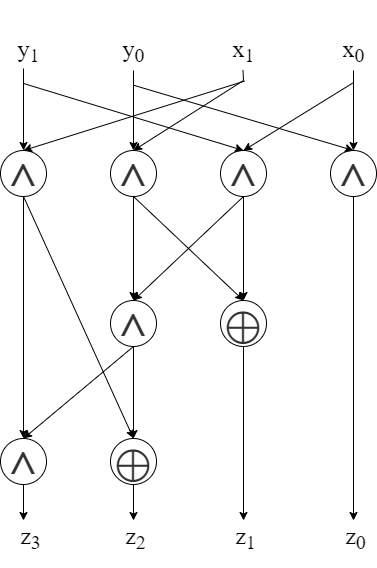
\includegraphics[scale=0.4]{diode.png}
\end{figure}

We have the following relation:
$$
z_0=y_0 \wedge x_0
$$
$$
u_1=y_1 \wedge x_0
$$
$$
u_2=y_0 \wedge x_1
$$
$$
u_3=y_1 \wedge x_1
$$
$$
z_1=u_1 \oplus u_2
$$
$$
u_4=u_1 \wedge u_2
$$
$$
z_2=u_3 \oplus u_4
$$
$$
z_3=u_3 \wedge u_4
$$

After simplifying the above formula, we get the following formula:
$$
\begin{aligned}
	z_0&=y_0 \wedge x_0\\
	z_1&=(y_1 \wedge x_0)\oplus(y_0 \wedge x_1)\\
	z_2&=(y_1 \wedge x_1)\oplus (y_1 \wedge x_0 \wedge y_0 \wedge x_1)\\
	z_3&=y_1 \wedge x_0 \wedge y_0 \wedge x_1
\end{aligned}
$$

\newpage
{\bf Problem 3.} Reduce the following Boolean function to the 3-SAT formula (remember the 3-
CNF form of 3-SAT):
$$
(x_1 \wedge x_2)\vee \neg(x_3 \wedge \neg x_4)
$$

\vskip 0.3 in

{\bf Answer 3.}
$$
\begin{aligned}
	&(x_1 \wedge x_2)\vee \neg(x_3 \wedge \neg x_4)\\
	=&(x_1 \wedge x_2) \vee (\neg x_3 \vee x_4)\\
	=&(x_1\vee \neg x_3 \vee x_4) \wedge (x_2\vee \neg x_3 \vee x_4)
\end{aligned}
$$

\vskip 0.3 in

{\bf Problem 4.} Design a probabilistic query algorithm to solve $x_1 \wedge x_2 $ with one query, such that probability of correct answer is more than 1/2.

\vskip 0.3 in

{\bf Answer 4.} Suppose we have $P(output 1)=p$, $P_{correct}=w$, we have the following situations.

1.$(x_1,x_2)=(1,1)$, then $w=p>\frac{1}{2}$.

2.$(x_1,x_2)=(1,0)$, then $w=1\times \frac{1}{2}+(1-p)\times \frac{1}{2}>\frac{1}{2}$, so $p<1$.

3.$(x_1,x_2)=(0,1)$, then the situation is similar to the above, we have $p<1$.

4.$(x_1,x_2)=(0,0)$, then $w=1>\frac{1}{2}$.

Let's take an example.
\begin{figure}[ht]
	\centering
	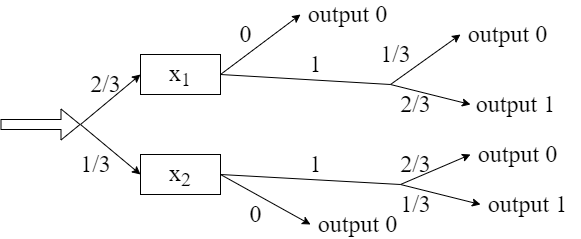
\includegraphics[scale=0.5]{example.png}
\end{figure}

1.$(x_1,x_2)=(0,0)$, then $P_{correct}=1$.

2.$(x_1,x_2)=(0,1)$, then $P_{correct}=\frac{2}{3}+\frac{1}{3}\times\frac{2}{3}=\frac{8}{9}$.

3.$(x_1,x_2)=(1,0)$, then $P_{correct}=\frac{1}{3}+\frac{2}{3}\times\frac{1}{3}=\frac{5}{9}$.

4.$(x_1,x_2)=(1,1)$, then $P_{correct}=\frac{1}{3}\times\frac{1}{3}+\frac{2}{3}\times\frac{2}{3}=\frac{5}{9}$.

The probabilistic query algorithm we designed satisfies the requirements.
\end{document}
